% Options for packages loaded elsewhere
\PassOptionsToPackage{unicode}{hyperref}
\PassOptionsToPackage{hyphens}{url}
\PassOptionsToPackage{dvipsnames,svgnames,x11names}{xcolor}
%
\documentclass[
  letterpaper,
  DIV=11,
  numbers=noendperiod,
  onecolumn]{scrartcl}

\usepackage{amsmath,amssymb}
\usepackage{iftex}
\ifPDFTeX
  \usepackage[T1]{fontenc}
  \usepackage[utf8]{inputenc}
  \usepackage{textcomp} % provide euro and other symbols
\else % if luatex or xetex
  \usepackage{unicode-math}
  \defaultfontfeatures{Scale=MatchLowercase}
  \defaultfontfeatures[\rmfamily]{Ligatures=TeX,Scale=1}
\fi
\usepackage{lmodern}
\ifPDFTeX\else  
    % xetex/luatex font selection
    \setmainfont[]{Lato}
\fi
% Use upquote if available, for straight quotes in verbatim environments
\IfFileExists{upquote.sty}{\usepackage{upquote}}{}
\IfFileExists{microtype.sty}{% use microtype if available
  \usepackage[]{microtype}
  \UseMicrotypeSet[protrusion]{basicmath} % disable protrusion for tt fonts
}{}
\makeatletter
\@ifundefined{KOMAClassName}{% if non-KOMA class
  \IfFileExists{parskip.sty}{%
    \usepackage{parskip}
  }{% else
    \setlength{\parindent}{0pt}
    \setlength{\parskip}{6pt plus 2pt minus 1pt}}
}{% if KOMA class
  \KOMAoptions{parskip=half}}
\makeatother
\usepackage{xcolor}
\setlength{\emergencystretch}{3em} % prevent overfull lines
\setcounter{secnumdepth}{-\maxdimen} % remove section numbering
% Make \paragraph and \subparagraph free-standing
\makeatletter
\ifx\paragraph\undefined\else
  \let\oldparagraph\paragraph
  \renewcommand{\paragraph}{
    \@ifstar
      \xxxParagraphStar
      \xxxParagraphNoStar
  }
  \newcommand{\xxxParagraphStar}[1]{\oldparagraph*{#1}\mbox{}}
  \newcommand{\xxxParagraphNoStar}[1]{\oldparagraph{#1}\mbox{}}
\fi
\ifx\subparagraph\undefined\else
  \let\oldsubparagraph\subparagraph
  \renewcommand{\subparagraph}{
    \@ifstar
      \xxxSubParagraphStar
      \xxxSubParagraphNoStar
  }
  \newcommand{\xxxSubParagraphStar}[1]{\oldsubparagraph*{#1}\mbox{}}
  \newcommand{\xxxSubParagraphNoStar}[1]{\oldsubparagraph{#1}\mbox{}}
\fi
\makeatother

\usepackage{color}
\usepackage{fancyvrb}
\newcommand{\VerbBar}{|}
\newcommand{\VERB}{\Verb[commandchars=\\\{\}]}
\DefineVerbatimEnvironment{Highlighting}{Verbatim}{commandchars=\\\{\}}
% Add ',fontsize=\small' for more characters per line
\usepackage{framed}
\definecolor{shadecolor}{RGB}{241,243,245}
\newenvironment{Shaded}{\begin{snugshade}}{\end{snugshade}}
\newcommand{\AlertTok}[1]{\textcolor[rgb]{0.68,0.00,0.00}{#1}}
\newcommand{\AnnotationTok}[1]{\textcolor[rgb]{0.37,0.37,0.37}{#1}}
\newcommand{\AttributeTok}[1]{\textcolor[rgb]{0.40,0.45,0.13}{#1}}
\newcommand{\BaseNTok}[1]{\textcolor[rgb]{0.68,0.00,0.00}{#1}}
\newcommand{\BuiltInTok}[1]{\textcolor[rgb]{0.00,0.23,0.31}{#1}}
\newcommand{\CharTok}[1]{\textcolor[rgb]{0.13,0.47,0.30}{#1}}
\newcommand{\CommentTok}[1]{\textcolor[rgb]{0.37,0.37,0.37}{#1}}
\newcommand{\CommentVarTok}[1]{\textcolor[rgb]{0.37,0.37,0.37}{\textit{#1}}}
\newcommand{\ConstantTok}[1]{\textcolor[rgb]{0.56,0.35,0.01}{#1}}
\newcommand{\ControlFlowTok}[1]{\textcolor[rgb]{0.00,0.23,0.31}{\textbf{#1}}}
\newcommand{\DataTypeTok}[1]{\textcolor[rgb]{0.68,0.00,0.00}{#1}}
\newcommand{\DecValTok}[1]{\textcolor[rgb]{0.68,0.00,0.00}{#1}}
\newcommand{\DocumentationTok}[1]{\textcolor[rgb]{0.37,0.37,0.37}{\textit{#1}}}
\newcommand{\ErrorTok}[1]{\textcolor[rgb]{0.68,0.00,0.00}{#1}}
\newcommand{\ExtensionTok}[1]{\textcolor[rgb]{0.00,0.23,0.31}{#1}}
\newcommand{\FloatTok}[1]{\textcolor[rgb]{0.68,0.00,0.00}{#1}}
\newcommand{\FunctionTok}[1]{\textcolor[rgb]{0.28,0.35,0.67}{#1}}
\newcommand{\ImportTok}[1]{\textcolor[rgb]{0.00,0.46,0.62}{#1}}
\newcommand{\InformationTok}[1]{\textcolor[rgb]{0.37,0.37,0.37}{#1}}
\newcommand{\KeywordTok}[1]{\textcolor[rgb]{0.00,0.23,0.31}{\textbf{#1}}}
\newcommand{\NormalTok}[1]{\textcolor[rgb]{0.00,0.23,0.31}{#1}}
\newcommand{\OperatorTok}[1]{\textcolor[rgb]{0.37,0.37,0.37}{#1}}
\newcommand{\OtherTok}[1]{\textcolor[rgb]{0.00,0.23,0.31}{#1}}
\newcommand{\PreprocessorTok}[1]{\textcolor[rgb]{0.68,0.00,0.00}{#1}}
\newcommand{\RegionMarkerTok}[1]{\textcolor[rgb]{0.00,0.23,0.31}{#1}}
\newcommand{\SpecialCharTok}[1]{\textcolor[rgb]{0.37,0.37,0.37}{#1}}
\newcommand{\SpecialStringTok}[1]{\textcolor[rgb]{0.13,0.47,0.30}{#1}}
\newcommand{\StringTok}[1]{\textcolor[rgb]{0.13,0.47,0.30}{#1}}
\newcommand{\VariableTok}[1]{\textcolor[rgb]{0.07,0.07,0.07}{#1}}
\newcommand{\VerbatimStringTok}[1]{\textcolor[rgb]{0.13,0.47,0.30}{#1}}
\newcommand{\WarningTok}[1]{\textcolor[rgb]{0.37,0.37,0.37}{\textit{#1}}}

\providecommand{\tightlist}{%
  \setlength{\itemsep}{0pt}\setlength{\parskip}{0pt}}\usepackage{longtable,booktabs,array}
\usepackage{calc} % for calculating minipage widths
% Correct order of tables after \paragraph or \subparagraph
\usepackage{etoolbox}
\makeatletter
\patchcmd\longtable{\par}{\if@noskipsec\mbox{}\fi\par}{}{}
\makeatother
% Allow footnotes in longtable head/foot
\IfFileExists{footnotehyper.sty}{\usepackage{footnotehyper}}{\usepackage{footnote}}
\makesavenoteenv{longtable}
\usepackage{graphicx}
\makeatletter
\newsavebox\pandoc@box
\newcommand*\pandocbounded[1]{% scales image to fit in text height/width
  \sbox\pandoc@box{#1}%
  \Gscale@div\@tempa{\textheight}{\dimexpr\ht\pandoc@box+\dp\pandoc@box\relax}%
  \Gscale@div\@tempb{\linewidth}{\wd\pandoc@box}%
  \ifdim\@tempb\p@<\@tempa\p@\let\@tempa\@tempb\fi% select the smaller of both
  \ifdim\@tempa\p@<\p@\scalebox{\@tempa}{\usebox\pandoc@box}%
  \else\usebox{\pandoc@box}%
  \fi%
}
% Set default figure placement to htbp
\def\fps@figure{htbp}
\makeatother

\KOMAoption{captions}{tableheading}
\makeatletter
\@ifpackageloaded{caption}{}{\usepackage{caption}}
\AtBeginDocument{%
\ifdefined\contentsname
  \renewcommand*\contentsname{Table of contents}
\else
  \newcommand\contentsname{Table of contents}
\fi
\ifdefined\listfigurename
  \renewcommand*\listfigurename{List of Figures}
\else
  \newcommand\listfigurename{List of Figures}
\fi
\ifdefined\listtablename
  \renewcommand*\listtablename{List of Tables}
\else
  \newcommand\listtablename{List of Tables}
\fi
\ifdefined\figurename
  \renewcommand*\figurename{Figure}
\else
  \newcommand\figurename{Figure}
\fi
\ifdefined\tablename
  \renewcommand*\tablename{Table}
\else
  \newcommand\tablename{Table}
\fi
}
\@ifpackageloaded{float}{}{\usepackage{float}}
\floatstyle{ruled}
\@ifundefined{c@chapter}{\newfloat{codelisting}{h}{lop}}{\newfloat{codelisting}{h}{lop}[chapter]}
\floatname{codelisting}{Listing}
\newcommand*\listoflistings{\listof{codelisting}{List of Listings}}
\makeatother
\makeatletter
\makeatother
\makeatletter
\@ifpackageloaded{caption}{}{\usepackage{caption}}
\@ifpackageloaded{subcaption}{}{\usepackage{subcaption}}
\makeatother

\usepackage{bookmark}

\IfFileExists{xurl.sty}{\usepackage{xurl}}{} % add URL line breaks if available
\urlstyle{same} % disable monospaced font for URLs
\hypersetup{
  pdftitle={Lab 1},
  pdfauthor={Paul \& Alex},
  colorlinks=true,
  linkcolor={blue},
  filecolor={Maroon},
  citecolor={Blue},
  urlcolor={Blue},
  pdfcreator={LaTeX via pandoc}}


\title{Lab 1}
\author{Paul \& Alex}
\date{2/18/25}

\begin{document}
\maketitle


\newpage

\section{Importance and Context}\label{importance-and-context}

In the United States, the last decades have seen an increasingly
polarized political climate. On a set of political questions measured by
the Pew Research Center, the average partisan gap between liberals and
conservatives has increased from 15 percentage points in 1994 to 36
percentage points in 2017.\footnote{Pew Research Center. ``The partisan
  divide on political values grows even wider.'' (2017).} At the same
time, national elections have been decided by increasingly narrow
margins. In both 2000 and 2016, the winner of the presidential election
lost the popular vote - an event that hadn't occurred previously since
1888. Responding to this environment, political campaigns have
increasingly emphasized voter turnout as a way to winning elections. The
question of how to motivate voters to show up at the polls has become
crucial to political strategists, as well as commentators and
researchers.

This analysis contributes to the discussion of voter motivation,
focusing on two emotions that frequently surface in discussions of the
2016 election: anger and fear. These two emotions are often cited in
explaining voter behavior, and they are key targets that political
advertisements are designed to play on. While anger and fear often go
hand in hand, they may differ in how well they motivate voter turnout,
as well as how they contribute to the overall polarization of society.
As a first step, this analysis aims to address the following research
question:

\begin{quote}
\emph{Was fear or anger more effective at causing voters to turn out in
the 2018 election?}
\end{quote}

The answer to this question could provide guidance to future political
campaigns hoping to increase voter turnout. It could also provide useful
background for governments that are interested civic participation. A
better understanding of the factors that polarize society, and how they
express themselves through the voting process, may also help those
hoping to counteract that polarization.

\section{Data and Methodology}\label{data-and-methodology}

Our analysis leverages data from the 2018 American National Election
Studies (ANES). This is an observational dataset, based on a sample of
respondents drawn from the YouGov platform. The YouGov panel is not
nationally representative, and consists of participants who sign up to
complete questionnaires in exchange for rewards. This dataset includes
1,500 individuals. We remove individuals who do not have election
turnout values reported in either 2016 or 2018, as well as individuals
who either report that they ``Do not know'', or ``Did not respond'' to
the key \emph{anger} or \emph{fear} survey questions.

As we report in Table~\ref{tbl-summary}, 70\% of ANES respondents report
that they voted in both the 2016 and 2018 elections. While turnout of
75\% might be expected in the presidential general, it is highly unusual
to have turnout this high in an off-cycle election. Also notable in this
data is that voting (or not voting) seems to be highly consistent over
time -- only 10\% of the respondents report taking a different action in
2016 compared to 2018.

To operationalize the concept of voter turnout, we consider changes in
voting behavior from 2016 to 2018. We refer to a change from not voting
to voting as a voting increase, and a change from voting to not voting
as a voting decrease. Although the net total of increases and decreases
may be interesting in some contexts, we focus on voting increases as our
main outcome variable. We believe that the ``new voters'' this variable
identifies are especially relevant to a study of increasing
turnout.\footnote{We exclude voters who were potentially too young to
  vote in 2016, resulting in fewer observations.}

As an alternative to our focus on voting increases, we considered
directly comparing voting rates in one fixed election. However, most
individuals maintain the same voting behavior over time, making it
difficult to relate a single voting decision to emotions in 2018.

\begin{longtable}[]{@{}lrr@{}}

\caption{\label{tbl-summary}Self-Reported Voting Behavior in 2016 and
2018}

\tabularnewline

\toprule\noalign{}
& Did not Vote 2018 & Voted 2018 \\
\midrule\noalign{}
\endhead
\bottomrule\noalign{}
\endlastfoot
Did not Vote 2016 & 0.19 & 0.04 \\
Voted 2016 & 0.05 & 0.72 \\

\end{longtable}

The survey includes questions about how angry and how afraid respondents
``feel about the way things are going in this country.'' Data is
reported on a 5-point Likert scale that ranges from 1 (``not at all'')
to 5 (``extremely''), and the same question is asked to each respondent.
These questions are about emotions in general, not necessarily emotions
relevant to voting, and the survey does not provide more information
about whether these emotions \emph{cause} voting behavior to change.

Because of the observational nature of the ANES data, we are not able to
directly measure whether anger or fear \emph{causes} voter turnout. We
can only check whether angry people or fearful people are more likely to
increase their voting behavior. Care must therefore be taken before
drawing causal conclusions based on our results.

\begin{figure}[t]

\centering{

\pandocbounded{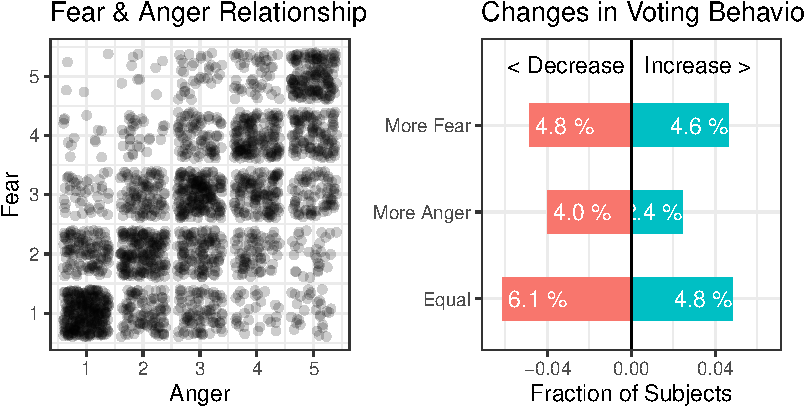
\includegraphics[keepaspectratio]{lab_1_example_solution_files/figure-pdf/fig-plots-1.pdf}}

}

\caption{\label{fig-plots}Voter Emotions and Voter Turnout. The red
series did not vote; the blue series did vote.}

\end{figure}%

The left panel of Figure~\ref{fig-plots} plots the empirical joint
distribution of respondents' feelings of fear and anger. The two
emotions are strongly related (Spearman correlation = 0.62) with 0.45 of
respondents reporting equal levels of anger and fear.

To compare the two emotions, we identify the respondents who are more
angry than afraid, and the respondents who are more afraid than angry.
While we could preserve more information by subtracting one measure from
the other, this would inappropriately impose a metric structure on these
ordinal variables.

We find that there are 825 people in the more-anger group and 495 people
in the more-fear group. The right panel of Figure~\ref{fig-plots} shows
the fraction of people in each group that reported an increase or
decrease in voting behavior. Subjects reporting equal emotions displayed
the most frequent changes in voting behavior, both increases and
decreases. Compared to the more-anger group, subjects in the more fear
group showed more frequent increases in voting behavior, and also more
frequent decreases. In line with our research question, we focus our
attention on the probability of increasing voting behavior within each
group.

Both our grouping variable and our outcome variable are measured at the
binary level. In this circumstance, common tests could include a
two-sample proportion test and Fisher's exact test. We proceed with a
two-sample t-test to demonstrate tools used in DATASCI 203. Given the
large sample sizes, the loss of accuracy from the t-test will be
negligible.

The null hypothesis of our t-test can be phrased as follows:

\begin{quote}
\textbf{Null Hypothesis:} \emph{The probability that a member of the
more-anger group shows an increase in voting is equal to the probability
that a member of the more-fear group shows an increase in voting}.
\end{quote}

In order for a t-test to produce reliable inference the following must
be true: the data must be drawn from an i.i.d. sample; measured on a
metric scale; and, be sufficiently normal that the central limit theorem
ensures convergence in distribution. We address each of these
requirements in turn.

First, data must be generated via an i.i.d. process. The ANES 2018 pilot
uses a panel of individuals from the YouGov platform. There is a
possibility that this introduces dependencies. For example, participants
may tell friends or family members about YouGov, resulting in a cluster
of individuals that give similar responses. Nevertheless, YouGov claims
to have millions of users, which suggests that links between individuals
should be rare.

Second, the outcome variable must be measured on a metric scale. In our
case, the presence of a voting increase is a binary variable. A binary
variable qualifies as metric as there is only a single interval, which
goes from zero to one.

Finally, the data must be sufficiently normal so that the CLT produces
convergence in distribution to a Gaussian distribution. The small number
of new voters can be understood as a positive skew in our turnout
variable (skewness = 4.72). Nevertheless, the large sample size suggests
that the sampling distribution of the statistic should be approximately
normal via the Central Limit Theorem.

\section{Results}\label{results}

\begin{Shaded}
\begin{Highlighting}[]
\NormalTok{test }\OtherTok{\textless{}{-}}\NormalTok{ anes }\SpecialCharTok{\%\textgreater{}\%} 
  \FunctionTok{filter}\NormalTok{(emotions }\SpecialCharTok{\%in\%} \FunctionTok{c}\NormalTok{(}\StringTok{"More Anger"}\NormalTok{, }\StringTok{"More Fear"}\NormalTok{)) }\SpecialCharTok{\%$\%} 
  \FunctionTok{t.test}\NormalTok{(voting\_change }\SpecialCharTok{==} \DecValTok{1} \SpecialCharTok{\textasciitilde{}}\NormalTok{ emotions)}
\end{Highlighting}
\end{Shaded}

The test yields evidence that more-fearful people are more likely than
more-angry people to increase voting behavior (t=-2.04, p=0.04). From a
practical perspective, this result appears potentially important. In the
more-anger group, 2.42 percent of participants are new voters. This
compares to 4.65 percent in the more-fear group, a difference of 2.23
percentage points. A difference of this size might typically be
considered a small effect, but in a highly competitive, polarized
electorate, even a small increase in message effectiveness may swing an
election.

Several limitations of our test affect the conclusions that may be drawn
from it. As mentioned above, we are only able to measure associations
between emotions and voting increases, not whether one feature causes
the other Additionally, the ANES data is not nationally representative,
suggesting that our results may not generalize to the US population.

\section{Discussion}\label{discussion}

This study found evidence that fear is more effective than anger at
driving voter turnout. The effect appears practically significant, with
more-fearful people estimated to be nearly twice as likely to be new
voters in 2018. While the absolute number of new voters remains small,
in a polarized and closely divided electorate, the difference of NA
percentage points may be enough to swing some close elections.

Our results may be of key interest to political campaigns, who have the
goal of tailoring advertisements to drive their supporters to the polls.
While this study addresses emotions in general, future studies may focus
directly on the emotional content of political advertisements. We are
especially interested in manipulating the emotional content of
advertisements in an experiment, providing a way to measure the causal
pathway from emotion to voting behavior. Finally, we hope that a general
understanding of emotions and voting can benefit society more broadly,
by revealing new ways to manage political polarization.




\end{document}
